\section{Funciones de error}

Entonces tomando como base el perceptrón, una vez obtenidas las salidas con una primera iteración nos daremos cuenta de que tan lejos o que tan cerca estuvimos de la respuesta correcta, con esto darnos la oportunidad de que pesos ajustar respecto a sus entradas, en la segunda iteración. Ahora para facilitarnos esto y tomando en cuenta que el entrenamiento consiste en varias iteraciones hasta llegar a aprender la tarea T, hacemos uso de una función de error que nos ayude a minimizar la diferencia de error en las salidas. 

Primero veamos el entrenamiento para una sola neurona, para esto haremos uso de la regla de aprendizaje del perceptrón (learning rule perceptron), donde para cada entrada, en la capa de salida se le calcula la desviación a la función objetivo. El cual utilizamos para ajustar los pesos del perceptrón (ver fig \ref{fig:errorP}). 

\begin{figure}[h]
 \centering
 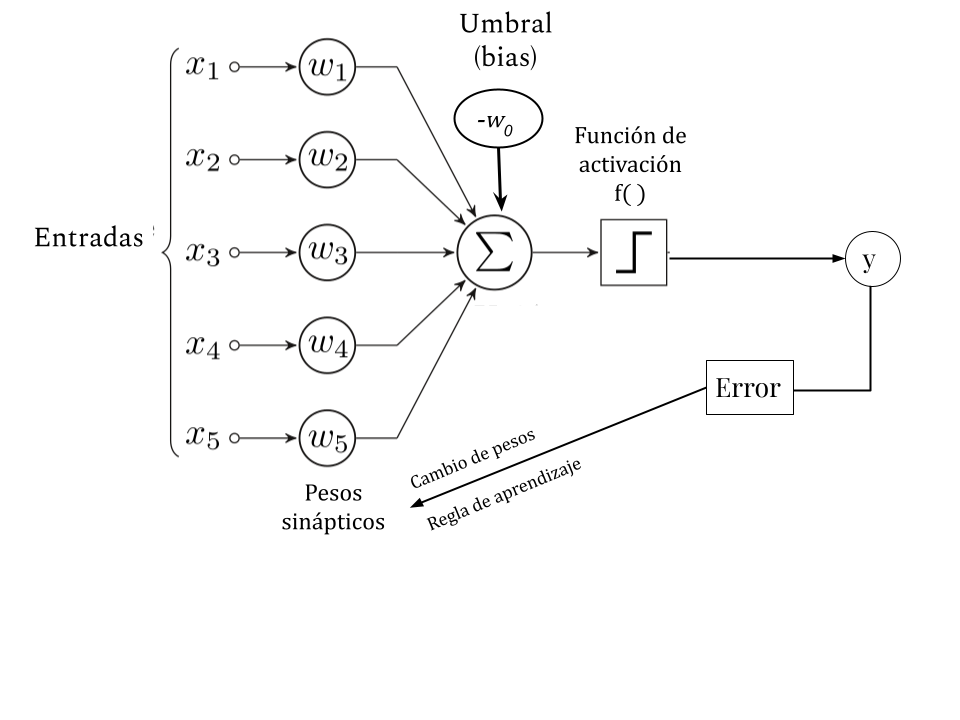
\includegraphics[scale=0.5]{../Figuras/ErrorPerceptron.png}
 \caption{Modelo estandar de un perceptrón.}
 \label{fig:errorP}
\end{figure}

Usualmente al principio del entrenamiento se asignan pesos aleatorios, a medida que avance el entrenamiento, se van modificando con cada iteración, así \(w_{i} \leftarrow w_{i} + \Delta w_{i}\). Esto con base a \emph{la regla de aprendizaje} donde: 

\begin{equation}
 \Delta w_{i} = \alpha(y - y_{out})x_{i}
\end{equation}

 
Con $y$ es la salida deseada, $y_{out}$ la salida generada, $\alpha$ la taza de aprendizaje (learning rate) y $x_{i}$ la entrada $i$. Lo que hace la taza de aprendizaje es moderar el grado en que los pesos son cambiados con cada iteración, se le asigna un valor muy pequeño (0.1 o 0.2) y conforme se logran ajustar los pesos se minimiza aún más. 


%Ahora supongamos que logramos que el perceptrón aprenda los datos
% de entrada, esto nos indica que $y = y_{out}$, haciendo que \
%(\Delta w_{i} = 0\), por tanto, ningún peso se actualice. En %nuestra etapa de validación, en un ejemplar nos de la salida $y = %-1$, cuando lo indicado es $1$. Entonces seguido de esa prueba %necesitamos hacer cambio de la taza de aprendizaje y renovación de %pesos aleatorios, para volver a ajustar los pesos correctamente y %no quede sobreajustada.


Para entrenar un perceptrón, utilizamos cualquier método de optimización de funciones para encontrar los parámetros $w$ que minimizan el error con alguna de las siguientes funciones de error:

\begin{description}
   
 \item \textbf{Diferencias al cuadrado}, también conocida como regla aprendizaje delta, es la suma de cuadrados de errores que se tuvieron con cada ejemplar el el conjunto de entranamiento. Los podemos decribir como: 
 
 \begin{equation}
   \dfrac{1}{2m}\sum_{m=0}^{M-1} (y_{m} - a_{m})^2
 \end{equation}
 
 con $y_{m}$ y $a{m}$, la salida obtenida dado un ejemplar $m$ y la salida correcta del ejemplar $m$ respectivamente.
 
 \item \textbf{Entropía cruzada.} Se usa para problemas de clasificación ya que su comportamiento es más suave (soft) y permite hacer clasificaciones más certeras. Se define como:

 \begin{equation}
  L (\Theta) = -\dfrac{1}{m}\sum_{M-1}^{m=0}(y^(m)log(a_{m}) + (1-y_{m}) log(1-a_{m})) 
 \end{equation}

\end{description}

Entonces juntando los conceptos que ya sabemos podemos describir el algoritmo de entrenamiento para el perceptrón de la siguiente forma:
\begin{enumerate}
 \item Iteramos sobre todos los ejemplares.
 \item Para cada ejemplar se calcula la función de propagación, es decir la suma ponderada.
 \item Se calcula la función de activación con esta suma.
 \item Se calcula la función de salida.
 \item Actualización de pesos de acuerdo a la regla de aprendizaje.
 \item Repetir de 1-6 hasta que los pesos nos satisfagan, un número de iteraciones establecidas.
\end{enumerate}


%Viéndolo como una especie de pseudocódigo lo podemos ver como:

%\begin{verbatim}
% Perceptron
%	input: Ejemplares
%	w: Pesos
%	y: correctas	
%	ta: taza de aprendizaje
%	o: respuestas predichas
%	
%Entrenamiento (input, w, y, ta):
%
%	for m in input: #iteramos sobre cada ejemplar
%		h = sum (w[m] * input[m]) #regla de propagación 
%		a = funcionActivacion(h) 
%		o[m] = 1 if (a*y[m]) > 0 else 0 #función de salida
%		w[m] = w[m] + (y[m] - o[m]) * ta * input[m] #regla de aprendizaje.
%
%\end{verbatim}


